\documentclass{article}

\textwidth=6.5in
\textheight=8.5in
\voffset=-54pt
\oddsidemargin=0in
\evensidemargin=0in
\setlength{\parskip}{8pt}
\setlength{\parindent}{0pt}

\usepackage{workbook}

\usepackage{handout}

\usepackage{exam}

\newcommand{\answerbox}[3][]{
    \fbox{\begin{minipage}[t][#2][c]{#3}
        #1
    \end{minipage}}
    }

\begin{document}

{\large \mbox{} \hfill \bf Name:\underline{\hspace{3in}}}\\[2pt]
{\mbox{} \hfill \it (Please write your name neatly in print.)}\\[12pt]
{\large \mbox{} \hfill \bf HUID:\underline{\hspace{3in}}}
 
\medskip
 
\noindent
{\large\bf
Exam 1 Practice 1\\
Math Mb Spring 2025}
\noindent


{\Large
\begin{center}\textbf{Directions---Please read carefully!} \end{center}}

This is a practice test. The same directions will appear on the actual exam, so read them carefully.

\hrulefill 


This exam is subject to the Harvard College Honor Code. No calculators or any other aids are permitted.  Please write as neatly as possible, as answers that can't be read can't be graded and thus can't receive credit. To receive full credit, you must show relevant working
and include units when appropriate. 

You have 120 minutes to complete this exam. 

You may ask for scratch paper if you need additional space to write, but it will not be scanned or graded. Make sure to include all relevant working in this exam booklet in the space provided for each question.

\begin{center}\textbf{Good luck!}\end{center}


\vfill

\centering{
\emph{As a member of Harvard College, I pledge that I will not give or receive assistance on this exam.}}
\vspace{0.3in}

{\large \mbox{} \hfill \bf Signature:\underline{\hspace{3in}}}
\thispagestyle{empty}

\newpage



\begin{enumerate}
\item Find the derivative of each function.
\begin{enumerate}
    \item $f(x)=2x^3\arcsin(\sqrt{x})$
    
    \begin{solution}
        \begin{align*}
        f'(x) &= \diff*{2x^3\arcsin(\sqrt{x})}{x} \\
        &= \left(\diff*{2x^3}{x}\right)\left(\arcsin(\sqrt{x})\right)+(2x^3)\left(\diff*{\arcsin(\sqrt{x})}{x}\right) \\
        &= (6x^2)\left(\arcsin(\sqrt{x})\right) + (2x^3)\Bigg(\frac{1}{\sqrt{1-(\sqrt{x})^2}}\Bigg)\left(\frac{1}{2\sqrt{x}}\right) \\
        &= 6x^2\arcsin(\sqrt{x}) + \frac{x^3}{\sqrt{x(1-x)}}
        \end{align*}

    \end{solution}
    \vfill
    \item $f(x)=\dfrac{x}{\cos(x^2)}+\tan(x^3)$
    
    \begin{solution}
        \begin{align*}
            f(x)&=\dfrac{x}{\cos(x^2)}+\tan(x^3) \\
            f(x)&=x\sec(x^2)+\tan(x^3) \\
            f'(x)&=\sec(x^2)+x\cdot \sec(x^2)\tan(x^2)\cdot2x+\sec^2(x^3)\cdot3x^2\\
            &= \sec(x^2) + 2x^2\sec(x^2)\tan(x^2)+ 3x^2\sec^2(x^3)
        \end{align*}
    \end{solution}
    \vfill
    \item $f(x)=x^{\cos x}$
    
    \begin{solution}
       \begin{align*}
           f(x)&=x^{\cos x}\\
           \ln[f(x)]&=\ln(x^{\cos x})\\
        \ln[f(x)]&=\cos x \cdot \ln x\\
        \dfrac{1}{f(x)}\cdot f'(x)&=-\sin x \cdot \ln x + \cos x \cdot \dfrac{1}{x} \\
        \dfrac{f'(x)}{f(x)}&=-\sin x \cdot \ln x + \dfrac{\cos x}{x}\\
     f'(x)&=f(x)\left[-\sin x \cdot \ln x + \dfrac{\cos x}{x}\right]\\
      f'(x)&=x^{\cos x}\left[-\sin x \cdot \ln x + \dfrac{\cos x}{x}\right]\\
       \end{align*} 
    \end{solution}
    \vfill
\end{enumerate}


\pspace{\newpage}


\item
  \label{spring2011-midterm1-2-expanded} \label{spring2011-midterm1-lemmings}
  % \points{14}

  Lemming populations experience huge oscillations in size over time.
  Scientists have determined that the density of lemmings in high-Arctic
  tundra in Greenland is roughly sinusoidal and periodic, with a period
  of 4 years.  When the population is most dense, there are roughly 1000
  lemmings per square km of tundra; when the population is least dense,
  there are roughly 20 lemmings per square km.

  \begin{enumerate}
  \item 
    \begin{problem}[\stretch{3}]      
      Write a a formula to model $L(t)$, the lemming density in the
      Greenland tundra at time $t$ (in years). At $t = 0$, the lemming population is at its peak density
      of 1000 lemmings per square kilometer.

      Accompany your formula with a rough sketch of the graph of $L(t)$.
    \end{problem}

    \begin{solution}
      Here's a sketch:
      \begin{center}
        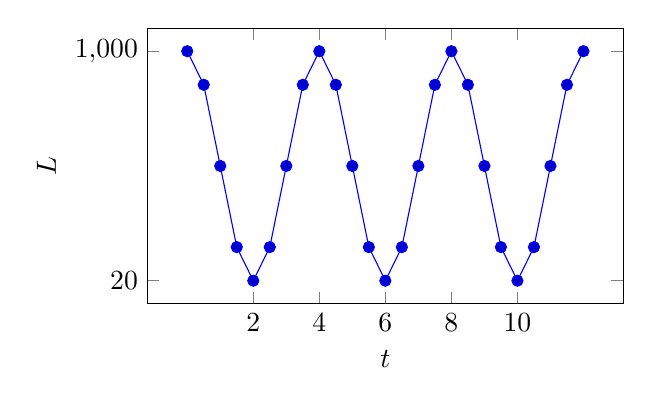
\begin{tikzpicture}
          \begin{axis}[xtick={2, 4, ..., 10}, ytick={20, 1000},
            xlabel=$t$, ylabel=$L$, width=3in, height=2in]
            \addplot+[domain=0:12] {490*cos(pi/2*deg(x))+510};
          \end{axis}
        \end{tikzpicture}
      \end{center}    
      To model this, it's helpful to find the amplitude, balance value, and
      period.  We are told that the period is 4; the amplitude is half of
      the difference between the highest value (1000) and lowest value (20),
      so the amplitude is 490.  The balance value is the value half-way
      between 1000 and 20, which is $\dfrac{1000 + 20}{2} = 510$.

      \ideas{\ding{52} We can check that our amplitude and balance
        value are consistent: if we add them, we should get the peak
        population (1000), and if we subtract the amplitude from the
        balance value, we should get the lowest population level (20).}

      Based on our sketch, it makes most sense to model with a cosine
      function, since the function we're modeling has a maximum at $t =
      0$.  So, the model is $L(t) = 490 \cos \left( \frac{2 \pi}{4} t
      \right) + 510$, which simplifies to $\boxed{L(t)=490 \cos \left(
          \frac{\pi}{2} t \right) + 510}$. 
    \end{solution}

  \item
    \begin{problem}[\vfill]
      At how many times between $t = 0$ and $t = 6$ is the lemming density
      equal to 90?
    \end{problem}

    \begin{solution}
      From the graph, we can see that there are 3 such times:
      \begin{center}
        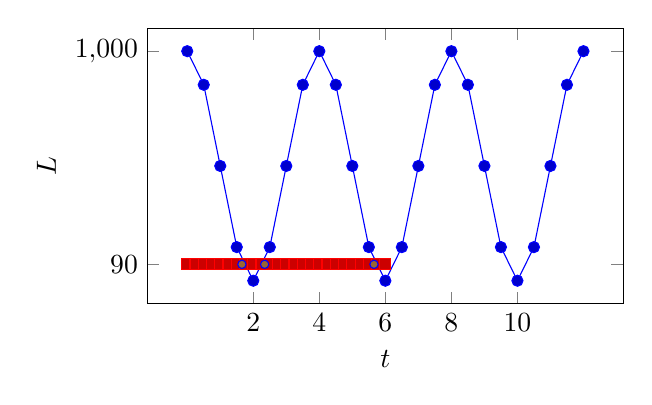
\begin{tikzpicture}
          \begin{axis}[xtick={2, 4, ..., 10}, ytick={90, 1000},
            xlabel=$t$, ylabel=$L$, width=3in, height=2in]
            \addplot+[domain=0:12] {490*cos(pi/2*deg(x))+510};
            \addplot+[domain=0:6] {90};
            \addplot+[only marks, mark=*, blue, mark size=1.5pt] coordinates
            {
              (1.65553, 90)
              (2.34447, 90)
              (5.65553, 90)
            };
          \end{axis}
        \end{tikzpicture}
      \end{center}    
    \end{solution}

    \pspace{\newpage}
    
\item
    \begin{problem}
        Solve for all times between $t=0$ and $t=6$ at which the lemming density is equal to 90. Give exact answers using inverse trigonometric functions.
    \end{problem}
    \pspace{\vfill}

\begin{solution}
    \begin{align*}
        490\cos(\tfrac{\pi}{2}t)+510 &= 90 \\
        490\cos(\tfrac{\pi}{2}t) &= -420 \\
        \cos(\tfrac{\pi}{2}t) &= -\tfrac{6}{7} \\
        \intertext{Based on the graph, we want the first three positive solutions, which would be }
        \tfrac{\pi}{2}t &= \arccos(-\tfrac{6}{7}),\ 2\pi- \arccos(-\tfrac{6}{7}),\ 2\pi + \arccos(-\tfrac{6}{7}) \\
        t &= \tfrac{2}{\pi}\arccos(-\tfrac{6}{7}),\ 4-\tfrac{2}{\pi}\arccos(-\tfrac{6}{7}),\ 4+\tfrac{2}{\pi}\arccos(-\tfrac{6}{7}).\\
        \intertext{Alternatively, we could have used $\arccos(\tfrac{6}{7})$ to express the solutions:}
        \tfrac{\pi}{2}t &= \pi-\arccos(\tfrac{6}{7}),\ \pi+\arccos(\tfrac{6}{7}),\ 3\pi - \arccos(\tfrac{6}{7}) \\
        t &=  2-\tfrac{2}{\pi}\arccos(\tfrac{6}{7}),\ 2+\tfrac{2}{\pi}\arccos(\tfrac{6}{7}),\ 6-\tfrac{2}{\pi}\arccos(\tfrac{6}{7}).
    \end{align*}

    We could have also found the first positive solution, $t=\tfrac{2}{\pi}\arccos(-\tfrac{6}{7})$ and then used the period, $4$, to derive the other solutions.
\end{solution}

  \end{enumerate}

  \item %Matt's question 
Write down the domain and range of the following functions.
        \begin{enumerate}
            \item $f(x) = \arctan(x)$ \hfill Domain: \solonly{$(-\infty, \infty)$}\hfill Range: \solonly{$(-\frac{\pi}{2}, \frac{\pi}{2})$}\hfill \phantom{.}

            \begin{solution}
                The domain of $f(x)= \arctan(x)$ is $(-\infty, \infty)$ (coming from the range of $\tan(x)$ and it's range is $\Big( -\dfrac{\pi}{2}, \dfrac{\pi}{2}\Big)$ coming from the restricted domain of $\tan(x)$.
            \end{solution}
            
            \vspace{.5 in}
            
            \item $f(x) = \arcsin(x)$ \hfill Domain: \solonly{$[-1, 1]$} \hfill Range: \solonly{$[-\frac{\pi}{2}, \frac{\pi}{2}]$} \hfill \phantom{.}

            \begin{solution}
                The domain of $f(x)= \arcsin(x)$ is $[-1, 1]$ (coming from the range of $\sin(x)$) and it's range is $\Big[ -\dfrac{\pi}{2}, \dfrac{\pi}{2}\Big]$ coming from the restricted domain of $\sin(x)$.
            \end{solution}
            
            \vspace{.5 in}
            \item $f(x) = \arccos(x)$ \hfill Domain: \solonly{$[-1, 1]$} \hfill Range: \solonly{$[0, \pi]$} \hfill \phantom{.}

            \begin{solution}
                The domain of $f(x)= \arccos(x)$ is $[-1, 1]$ (coming from the range of $\cos(x)$) and it's range is $[0,\pi]$ coming from the restricted domain of $\cos(x)$.
            \end{solution}
            
            \vspace{.5 in}

        \end{enumerate}

\pspace{\newpage}
\item \label{spring2011-midterm1-7}

  % \points{8}

  Let $(a, b)$ be
  the point on the circle of radius $7$ centered at $(0, 0)$ shown below.

  \begin{tikzpicture}
      \begin{axis}[
      xlabel=$x$, ylabel=$y$,
      xmin=-8, xmax=8, ymin=-8, ymax=8,
      xtick={-7,7}, ytick={-7,7},
      axis equal image,
      clip=false,
      width=2.75in
      ]
        \addplot[domain=0:360] ({7*cos(x)},{7*sin(x)});
        \addplot[closed] coordinates {(-3.5,-6.06)};
        \addplot[->,domain=0:240] ({0.7*cos(x)},{0.7*sin(x)});
        \draw (axis cs:0,0) -- (axis cs:-3.5,-6.06);
        \node at (axis cs:-0.7,1) {$\theta$};
        \node[below left] at (axis cs:-3.5, -6.06) {$(a, b)$};
      \end{axis}
  \end{tikzpicture}

  \begin{enumerate}
  \item
    \begin{problem}[\stretch{2}]
      Sketch the tangent line to the circle at the point $(a, b)$.  Use
      implicit differentiation to find the slope of this line. 

      {\it Your answer will be in terms of $a$ and $b$.}
    \end{problem}

    \begin{solution}
      We are looking for $\dfrac{dy}{dx}$ at the point $(a, b)$.  To
      start, we need the equation of the circle, which is
      \begin{align*}
        x^2 + y^2 & = 7^2 \\
        \intertext{Now, we'll take the derivative of both sides with
          respect to $x$:} 
        2x + 2y \frac{dy}{dx} & = 0 \\
        \intertext{Next, we'll solve for $\dfrac{dy}{dx}$:}
        \frac{dy}{dx} & = -\frac{x}{y} \\
      \end{align*}
      Therefore, at the point $(a,b)$, the slope is
      $\boxed{-\frac{a}{b}}$. 
    \end{solution}

  \item
    \begin{problem}[\vfill]
      We have drawn the line segment through $(0,0)$ and $(a,b)$.  Let
      $\theta$ be the angle shown, whose terminal ray is along this line.  Find the value of $\tan \theta$.
    \end{problem}

    \begin{solution}
      $\displaystyle \tan(\theta) = \frac{\sin(\theta)}{\cos(\theta)} =
      \frac{b/7}{a/7} = \boxed{\frac{b}{a}}$.
    \end{solution}

  
  \item 
  
  If $\theta$ is in the interval $[0, 2 \pi]$, which of the
    following are equal to $\theta$?  Circle \textbf{all}.
    \begin{multicols}{2}
      \begin{enumerate}[label=\protect\maybecircle{\Alph*.}]
      \plainitem $\displaystyle \arccos \left( \frac{a}{7} \right)$
      \plainitem $\displaystyle \pi + \arccos \left( \frac{a}{7} \right)$
      \circleitem $\displaystyle 2\pi - \arccos \left( \frac{a}{7} \right)$
      \plainitem $\displaystyle - \arccos \left( \frac{a}{7} \right)$
      \end{enumerate}
    \end{multicols}

    \begin{solution}
      All of the choices involve $\displaystyle \arccos \left( \frac{a}{7}
      \right)$, so let's first figure out what this angle is.  By
      definition, $\displaystyle \arccos \left( \frac{a}{7} \right)$ is
      the angle in $[0, \pi]$ whose cosine is $\dfrac{a}{7}$.  In other
      words, $\displaystyle \arccos \left( \frac{a}{7} \right)$ must be
      the angle shown in red in the following picture:
      \begin{center}
        \includegraphics[width=1.5in]{Old Assessments/Midterms/spring2011-midterm1-arccos.pdf}
      \end{center}
      Then, by symmetry, we can see that $\theta$ (the angle in black) is
      $\displaystyle 2 \pi - \arccos \left( \frac{a}{7} \right)$.
    \end{solution}

    \pspace{\newpage}

  \end{enumerate}

\item 
% \points{10}

\begin{problem}
At a given instant, a helicopter is flying 500 meters directly over an observer on the ground. The helicopter is flying horizontally at a constant rate of 50 meters per second. After 10 seconds, how fast is the angle $\theta$ between the vertical and the observer's line of sight to the helicopter changing in radians per second?

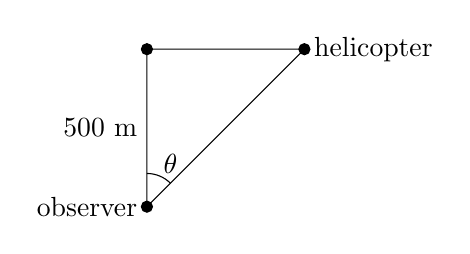
\begin{tikzpicture}
        \coordinate (A) at (2, 2);
        \draw (0,0) -- node[left]{500 m} (0, 2) -- (2,2) -- (0,0);
        \draw (0,12pt) arc[radius=12pt, start angle=90, end angle=45]
            node[above]{$\theta$};  
        \filldraw (0, 0) circle(2pt) node[left] {observer};
        \filldraw (0,2) circle(2pt);
        \filldraw (2,2) circle (2pt) node[right] {helicopter};
\end{tikzpicture}
          
\end{problem}

\pspace{\newpage}

\begin{solution}
    \textcolor{red}{Let's start with sketching our snapshot and generic pictures of situation.}
    Our snapshot shows the situation at the time that we care about and the generic picture applies at any time.

    After 10 seconds, the helicopter has travelled (50 meters/second)(10 seconds) = 500 meters.

\begin{center}
        \begin{tabular}{ccc}
          \emph{Snapshot} & \hspace{0.25in} & \emph{Generic} \\
          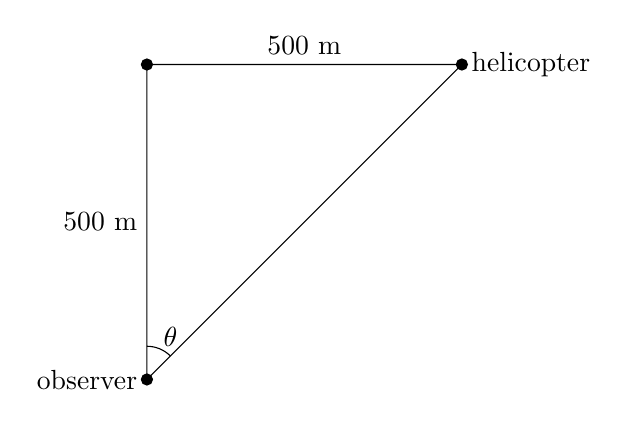
\begin{tikzpicture}
            \coordinate (A) at (4, 4);
            \draw (0,0) -- node[left]{500 m} (0, 4) -- node[above]{500 m} (4,4) -- (0,0);
            \draw (0,12pt) arc[radius=12pt, start angle=90, end angle=45]
            node[above]{$\theta$};  
            \filldraw (0, 0) circle(2pt) node[left] {observer};
            \filldraw (0,4) circle(2pt);
            \filldraw (4,4) circle (2pt) node[right] {helicopter};
        \end{tikzpicture} &&
          \begin{tikzpicture}
            \coordinate (A) at (4, 4);
            \draw (0,0) -- node[left]{500 m} (0, 4) -- node[above]{x} (4,4) -- (0,0);
            \draw (0,12pt) arc[radius=12pt, start angle=90, end angle=45]
            node[above]{$\theta$};  
            \filldraw (0, 0) circle(2pt) node[left] {observer};
            \filldraw (0,4) circle(2pt);
            \filldraw (4,4) circle (2pt) node[right] {helicopter};
        \end{tikzpicture}
        \end{tabular}
      \end{center}
    In our generic picture, we'll let $x$ be the distance traveled by the helicopter since the instant at which it was directly over the observer.

    \textcolor{red}{Next, we'll identify what we know and what we want to know.}

    \textbf{What we know:} $\frac{dx}{dt}=50$\\
    \textbf{What we want to know:} $\frac{d\theta}{dt}$ when $t=10$ seconds.

    \textcolor{red}{Next, we'll write an equation relating our variables.}

    Because the rate we know if $\frac{dx}{dt}$ and the rate we want is $\frac{d\theta}{dt}$, we should write an equation relating $x$ and $\theta$.

    \textbf{Equation relating our variables:} $\tan \theta=\frac{x}{500}$.

    \textcolor{red}{Next, we'll differentiate our equation. Because we want $\frac{dx}{dt}$, we'll differentiate with respect to $t$.}

    \begin{align}
        \frac{d}{dt}\left(\tan \theta \right) &= \frac{d}{dt} \left( \frac{x}{500} \right) \\
        \sec^2\theta \cdot \frac{d\theta}{dt} &= \frac{1}{500} \cdot \frac{dx}{dt}
    \end{align}

    \textcolor{red}{Finally, we'll plug in our snapshot information and solve for what we're looking for. (In this case, $\frac{d\theta}{dt}$.)}

    \[\sec^2\theta \cdot \frac{d\theta}{dt} = \frac{1}{500} \cdot 50\]

    Since the triangle in our snapshot is an isosceles triangle, at this moment, $\theta=\frac{\pi}{4}$. Plugging this into our above equation,

    \begin{align}
        \sec^2(\frac{\pi}{4}) \cdot \frac{d\theta}{dt} &= \frac{1}{500} \cdot 50\\
        \frac{1}{\cos^2(\frac{\pi}{4})} \cdot \frac{d\theta}{dt} &= \frac{1}{500} \cdot 50\\
        \frac{1}{(\frac{1}{\sqrt{2}})^2} \cdot \frac{d\theta}{dt} &= \frac{1}{500} \cdot 50\\
        \frac{1}{\frac{1}{2}} \cdot \frac{d\theta}{dt} &= \frac{1}{500} \cdot 50\\
        2 \cdot \frac{d\theta}{dt} &= \frac{1}{500} \cdot 50
    \end{align}

    So $\boxed{\frac{d\theta}{dt} = \frac{1}{20}} \text{ radians/second}$.

    

    
\end{solution}

\item \label{inverse-trig-composition-2}
  % \points{10}  
 
 Let $f(x) = \tan(\arccos x)$.

  \begin{enumerate}
  \item
    \begin{problem}[\vfill]
      Evaluate $f \left( - \frac{\sqrt{2}}{2} \right)$ or explain why it is
      undefined. 
    \end{problem}

    \begin{solution}
      By definition, $\arccos \left( - \frac{\sqrt{2}}{2} \right)$ is the
      angle in $[0, \pi]$ whose cosine is $- \frac{\sqrt{2}}{2}$; this
      angle is $\frac{3 \pi}{4}$.  So, $f \left( - \frac{\sqrt{2}}{2}
      \right) = \tan \frac{3 \pi}{4} = \boxed{-1}$. 
    \end{solution}

  \item
    \begin{problem}[\vfill]
      Evaluate $f(0)$ or explain why it is undefined.
    \end{problem}

    \begin{solution}
      By definition, $\arccos 0$ is the angle in $[0, \pi]$ whose cosine
      is $0$; this angle is $\frac{\pi}{2}$.  So, $f(0) = \tan
      \frac{\pi}{2}$, which is \fbox{undefined}.
    \end{solution}

  \item
    \begin{problem}[\vfill]
      Evaluate $f(\pi)$ or explain why it is undefined. 
    \end{problem}

    \begin{solution}
      $\arccos(\pi)$ is undefined because there is no angle in $[0, \pi]$
      whose cosine is $\pi$ (the cosine of any angle is at most 1).  So,
      $f(\pi)$ is \fbox{undefined}.
    \end{solution}

  \item
    \begin{problem}[\vfill]
      What is the domain of $f(x)$?
    \end{problem}

    \begin{solution}
      The domain of $f(x)$ is \fbox{all numbers in $[-1, 1]$ except 0}.
      We can only take $\arccos$ of numbers in $[-1, 1]$; if we take the
      $\arccos$ of any number in $[-1, 1]$, we end up with a number in
      $[0, \pi]$, and we can then take the tangent of that \emph{except}
      if it is $\frac{\pi}{2}$ (which is $\arccos 0$).
    \end{solution}

  \item
    \begin{problem}[\vfill]
      What is the range of $f(x)$?
    \end{problem}

    \begin{solution}
      The domain is all numbers in $[-1, 1]$ except 0; if we plug such
      numbers into $\arccos$, then we get all numbers in $[0, \pi]$ except
      for $\frac{\pi}{2}$.  If we then plug these numbers into $\tan$, we
      get \fbox{all real numbers}.
    \end{solution}
    \end{enumerate}

\pspace{\newpage}
  
\item
  \label{spring2011-mb-midterm1-8} 
  % \points{14}

  The pressure $P$ (in atmospheres) and volume $V$ (in liters) of a
  certain quantity of gas are related by Van der Waal's equation
  \begin{equation*}
    \label{spring2011-mb-midterm1-8-eq}
    \left(P + \frac{18}{V^2}\right) (V-1) = 6.
  \end{equation*}

  \begin{enumerate}

  % \item
  %   \begin{problem}[1.5in]
  %     We find that when the pressure is 1 atmosphere, the volume is 3
  %     liters.  Use this to find the value of the constant $C$.  We'll use this value of $C$ for the rest of the problem.
  %   \end{problem}

  %   \begin{solution}
  %     We know that, when $P = 1$, $V = 3$.  Plugging $P = 1$ and $V = 3$
  %     into the equation
  %     \begin{align*}
  %       \left(P + \frac{18}{V^2}\right) (V-1) &= C \\
  %       \intertext{gives}
  %       \left( 1 + \frac{18}{3^2} \right) (3 - 1) &= C \\
  %       \boxed{6} &= C
  %     \end{align*}
  %   \end{solution}

  \item
    \begin{problem}[\stretch{3}]
      The graph of the relationship between the volume and the pressure of the gas is shown below.  Find 
      $\frac{dV}{dP} $ when the pressure is 1 atmosphere and the volume is 3 liters. Include units.

      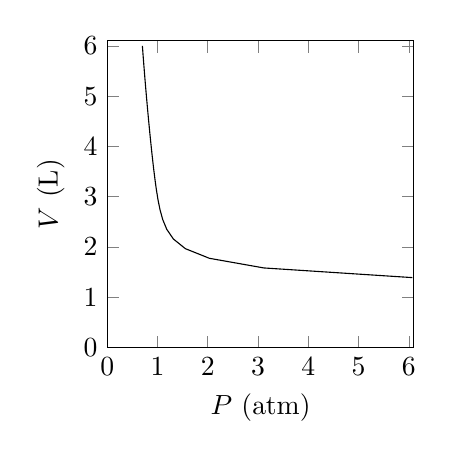
\begin{tikzpicture}
          \begin{axis}[
          xlabel=$P$ (atm), ylabel=$V$ (L),
          xmin=0, xmax=6.1, ymin=0, ymax=6.1,
          axis equal image,
          xtick distance=1, ytick distance=1,
          width=2.5in
          ]
          \addplot[domain=1.39:6] (6/(x-1)-18/x^2,x);
          \end{axis}
      \end{tikzpicture}
    \end{problem}

    \begin{solution}
      Using the $C$ we found, we know that
      \begin{align*}
        \left(P + \frac{18}{V^2}\right) (V-1) &= 6 \\
        \intertext{We want to find $\frac{dV}{dP}$, and it doesn't look
          easy to solve for $V$ in terms of $P$.  Instead, let's use
          implicit differentiation.  Since we want
          $\frac{dV}{d\color{red}P\color{black}}$, we'll differentiate
          both sides with respect to \color{red}$P$\color{black}:}
        \frac{d}{d\color{red}P\color{black}}
        \left(\fcolorbox{green}{white}{$\displaystyle  \left(P+ 18 V^ {
                -2} \right)$}\cdot
          \fcolorbox{green}{white}{$\displaystyle
            \left(V-1\right)$}\right) &=
        \frac{d}{d\color{red}P\color{black}} 6\\
        \left(P+ 18 V^ { -2} \right)\cdot \frac{d}{dP}\left(V-1\right)+
        \frac{d}{dP}\left(P+ 18 V^ { -2} \right)\cdot \left(V-1\right) &=
        0 \\
        \left(P+ 18 V^ { -2} \right)\cdot \frac{dV}{dP}+ \left(1+ 18\cdot
          \frac{d}{dP} \left(\fcolorbox{red}{white}{$\displaystyle
              \fcolorbox{blue}{white}{$\displaystyle  V$}^ { -2}
              $}\right)\right)\cdot \left(V-1\right) &= 0 \\
        \left(P+ 18 V^ { -2} \right)\cdot \frac{dV}{dP}+ \left(1-36 V^ {
            -3} \cdot \frac{dV}{dP}\right)\cdot \left(V-1\right) &= 0 \\
        \intertext{We care about what happens when $P = 1$ and $V = 3$, so
          let's plug these values in:} \left( 1 + \frac{18}{3^2} \right)
        \frac{dV}{dP} + \left(1 -
          \frac{36}{3^3} \frac{dV}{dP} \right) 2 &= 0 \\
        3 \frac{dV}{dP} + 2 \left( 1 - \frac{4}{3} \frac{dV}{dP} \right) &= 0 \\
        \frac{1}{3} \frac{dV}{dP} + 2 &= 0 \\
        \frac{1}{3} \frac{dV}{dP} &= -2 \\
        \frac{dV}{dP} &= \boxed{-6\text{ liter/atm}}
      \end{align*}

      (Note that, from the picture given, $\frac{dV}{dP}$ should be
      negative when $P = 1$.)
    \end{solution}

  % \item \label{spring2011-mb-midterm1-8-tangent-line}
  %   \begin{problem}[\vfill]
  %     Find the linear function $L(P)$ that best approximates $V$ as a function of
  %     $P$ when $P$ is close to 1.

  %     % {\it Note that this is another way of asking you to find the
  %     %   equation of the tangent line to the implicitly defined curve at
  %     %   the point when $P=1$.}
  %   \end{problem}

  %   \begin{solution}
      % We just found that the slope of the tangent line was $-6$, and we
      % know $(1, 3)$ is a point on the tangent line, so the equation of the
      % line is $\boxed{V - 3 = - 6 (P - 1)}$.
  %   \end{solution}

  \item
    \begin{problem}[\vfill]
     Approximate the volume when the pressure is 1.01 atmospheres.
    \end{problem}

    \begin{solution}
    We just determined that, when $P=1$, $\frac{dV}{dP}=-6\text{ liter/atm}$. If the pressure increases by $0.01$ atm, the volume would change by approximately $(-6\text{ liter/atm})(0.01\text{ atm})=-0.06$ liter. This means that the new volume would be approximately $3-0.06=2.94$ liters.
      % We just found that the slope of the tangent line was $-6$, and we
      % know $(1, 3)$ is a point on the tangent line, so the equation of the
      % line is $\boxed{V - 3 = - 6 (P - 1)}$.
      % The tangent line we just found was $V = - 6 (P - 1) + 3$.  This
      % should be a good approximation for the actual curve near the point
      % $(1, 3)$, so $ - 6 (P - 1) + 3$ is a good approximation for the
      % actual volume when $P$ is near 1.  In particular, if we plug in $P =
      % 1.01$, we get that the volume is approximately $ - 6 (1.01 - 1) + 3
      % = - 6 \cdot 0.01 + 3 = \boxed{2.94}$.

      % (Again, this is reasonable from the picture: when $P$ is slightly
      % bigger than $1$, $V$ should be slightly smaller than $3$.)
    \end{solution}

  \end{enumerate}
%  \item \label{spring2014-mb-midterm1-3-modified} 
%   % \points{20} 
% \begin{problem}
%     To determine the height of a mountain peak above a level plain, the angle of elevation to the top of the mountain is measured to be $32$  degrees. 1000 feet closer to the mountain along the plain the angle of elevation to the peak is $35$ degrees. Find the height of the mountain. Give an exact answer. You do not need to evaluate trigonometric functions of non-special angles.
% \end{problem}

% \pspace{\stretch{2.5}}

% \begin{solution}

% Let $h$ be the height of the mountain peak from the plain. Then, according to the information given, we have the following picture:

%     \begin{center}
%         \begin{tikzpicture}[x=1.5cm, y=1.5cm]
%           \coordinate (ground) at (0, -0.4); %
%           \coordinate (A) at (0, 0); %
%           \coordinate (B) at (1, 0); %
%           \coordinate (C) at (4, 2); %
%           \coordinate (D) at (4, 0);
%           \draw[very thick] (A) node[below left] {$A$} -- 
%           (C) node[above] {$C$} -- (D) node[below left] {$D$}; %
%           \draw[very thick] (B) node[below left] {$B$} -- (C) -- (D); %
%           \draw[very thick] (A) -- (D);
%           \draw[decorate, decoration={brace, mirror}] 
%           ($(A |- ground) - (0,2pt)$) -- node[below, yshift=-2pt]
%           {$1000$ feet} ($(B |- ground) - (0, 2pt)$); %
%           \draw[decorate, decoration={brace, mirror}] 
%           ($(B |- ground) - (0,2pt)$) -- node[below, yshift=-2pt]{$x$} 
%           ($(C |- ground) - (0,2pt)$); %
%           \draw (C |- A) -- (C); %
%           \draw pic[draw=red, "$\ang{32}$", angle radius = 20, angle eccentricity = 1.5] {angle=D--A--C};
%           \draw pic[draw=blue, "$\ang{35}$", angle radius = 20, angle eccentricity = 1.5] {angle=D--B--C};
%           \draw[decorate, decoration={brace}] ($(C)+(2pt,0)$) -- 
%           node[right,xshift=2pt]{$h$} ($(D)+(2pt,0)$);
%         \end{tikzpicture}
%       \end{center}

% Since triangle $CAD$ is a right triangle, we know that:

% \begin{align*}
%     \tan(32^{\circ})&=\frac{h}{x+1000}\\
%     h&=(x+1000)\tan(32^{\circ}) \tag{1}
% \end{align*}

% Similarly, since triangle $CBD$ is a right triangle, we know that:

% \begin{align*}
%     \tan(35^{\circ})&=\frac{h}{x}\\
%     h&=x\tan(35^{\circ}) \tag{2}
% \end{align*}

% Setting equations (1) and (2) equal to each other, we get:

% \begin{align*}
%     x\tan(35^{\circ})&= (x+1000)\tan(32^{\circ})\\
%     x\tan(35^{\circ}) &= x\tan(32^{\circ}) + 1000\tan(32^{\circ}) \\
%     x\tan(35^{\circ}) - x\tan(32^{\circ}) &=1000\tan(32^{\circ})\\
%     x(\tan(35^{\circ})-\tan(32^{\circ}))&=1000\tan(32^{\circ})\\
%     x&=\frac{1000\tan(32^{\circ})}{\tan(35^{\circ})-\tan(32^{\circ})}
% \end{align*}

% Plugging this value of $x$ into equation (2), we get:

% $$\boxed{h=\frac{1000\tan(32^{\circ})\tan(35^{\circ})}{\tan(35^{\circ})-\tan(32^{\circ})} \text{ feet}}$$

% \end{solution}

\pspace{\newpage}

\item 
\begin{problem}
You are driving north along a straight road. 
To your right, there is an 30-foot-wide billboard. The left edge
of the billboard is 
10 feet from the road. At what distance $x$ from the billboard
is your viewing angle $\theta$ at a maximum?


\includegraphics[scale=0.3]{assessments/Exam 1/Practice Exams/billboard.png}
\end{problem}
\pspace{\stretch{3}}

\begin{solution}
First, we need to express $\theta$, the quantity we want to maximize, in terms of $x$. We can express $\theta$ as
$\theta = \alpha - \beta$, where $\alpha$ is the angle formed by the side of the road and the line of sight to the right side of the billboard and $\beta$ is the angle formed by the side of the road and the line of sight to the left side of the billboard.

Using trigonometry, we know that 
\[\tan(\alpha)=\dfrac{40}{x} \quad \text{and} \quad 
\tan(\beta)=\dfrac{10}{x},\] 
therefore 
\[\alpha = \arctan\biggl(\dfrac{40}{x}\biggr) \quad \text{and} 
\quad \beta = \arctan\biggl(\dfrac{10}{x}\biggr).\]

This means that we can express $\theta$ as a function of $x$ 
on the domain $x > 0$ as follows.
\[\theta = \arctan\biggl(\dfrac{40}{x}\biggr) - 
\arctan\biggl(\dfrac{10}{x}\biggr)\]

To maximize this function, let's first find the critical points
by finding the derivative.
\begin{align*}
    \dfrac{d\theta}{dx} &= \left(\dfrac{1}{1+(\frac{40}{x})^2}\right)
    \left(-\dfrac{40}{x^2}\right) - \left(\dfrac{1}{1+(\frac{10}{x})^2}\right)
    \left(-\dfrac{10}{x^2}\right) \\
    \intertext{To help us solve for the critical points,
    let's simplify the derivative.}
    \dfrac{d\theta}{dx} &= \dfrac{-40}{x^2 + 1600} + \dfrac{10}{x^2 + 100} \\[5pt]
    &= \dfrac{-40(x^2+100)+10(x^2+1600)}{(x^2+1600)(x^2+100)}\\[5pt]
    &= \dfrac{-30x^2+12000}{(x^2+85^2)(x^2+40^2)} \\[5pt]
    &= \dfrac{-30(x^2-400)}{(x^2+85^2)(x^2+40^2)} \\[5pt]
    &= \dfrac{-30(x-20)(x+20)}{(x^2+85^2)(x^2+40^2)}
\end{align*}

To determine the critical points, we need to look for where 
$\frac{d\theta}{dx}$ is zero or undefined. $\frac{d\theta}{dx}$ is zero when the numerator is zero, so when $x=\pm 20$.
$\frac{d\theta}{dx}$ is undefined when the denominator is zero, which never happens. 
Since the domain is $x>0$, the only critical point is $x=20$. 

Now we need to determine whether the global maximum is achieved
at 
$x=20$, which, since it is the only critical point, we can do by considering where $\theta$ is increasing and decreasing. Since $\frac{d\theta}{dx}$
is positive when $x<20$ and negative when $x>20$, $\theta$
increases when $0<x<20$ and decreases when $x>20$, and therefore
the maximum value of $\theta$ is achieved when $x=20$.

The maximum viewing angle occurs when you are $20$ feet away
from the billboard. 


\end{solution}

\probonly{
\newpage
\textit{This page has been intentionally left blank for scratch work. No work on this page will be graded.}
}
\end{enumerate}
\end{document}
